\section{NAT traversing}
\label{sec: NatTraversing}

Before the PPETP protocol could be utilized, it's necessary a registration phase to a server; how this procedure is accomplished is out of the scope of PPETP \footnote{I.e. with HTTP or RTP}. In this phase the server transmit to the new peer a list of other peer yet registered for the desired media and a set of configuration information (i.e. as a XML file)(see fig. \ref{fig:text_phase}). At this point a new PPETP session could be initialized. 
\begin{figure}[htbp]
	\centering
		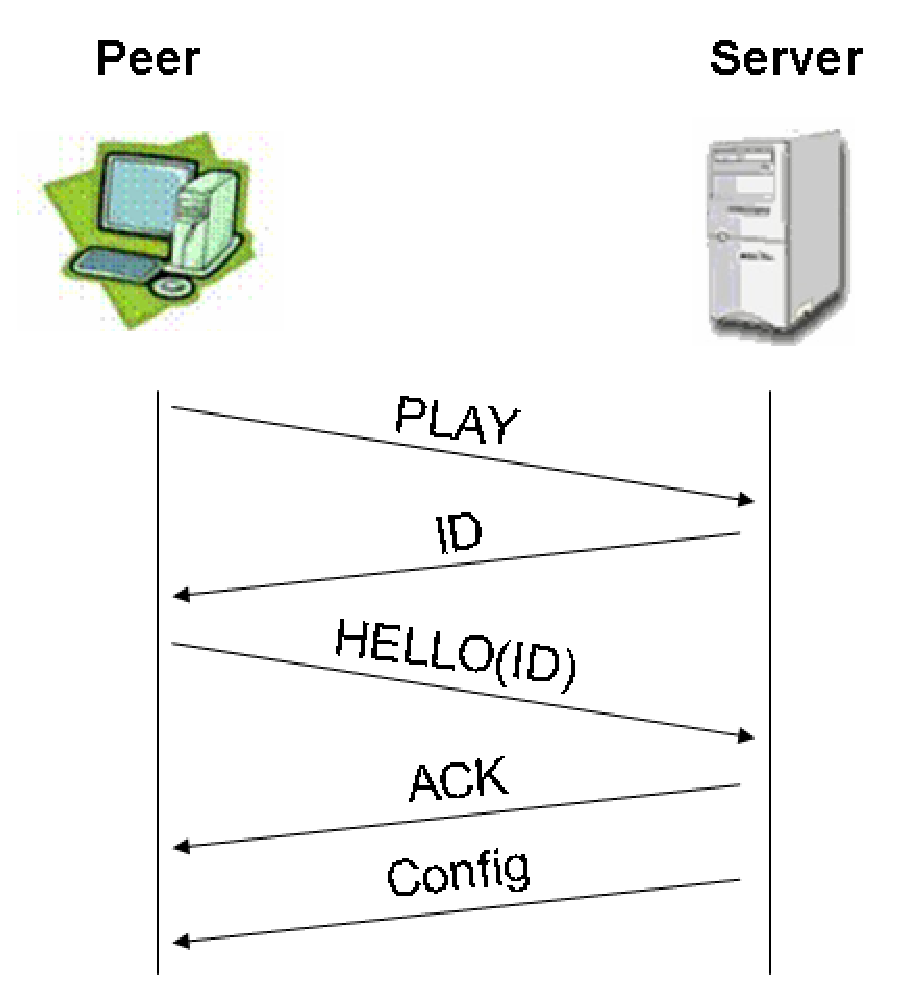
\includegraphics[scale=0.5]{text_phase.eps}
	\caption[Text-Based handshake]{Text-Based handshake}
	\label{fig:text_phase}	
\end{figure}

The first operation for the NAT traversing is to guarantee the achievablety(??) between the server and the peer. To obtain this, the peer send two PPETP HELLO packet to the server. The first packet is sent from the PPETP write port (is the session port + 1) to the PPETP session port of the server; in this way the NAT register the pair <Peer\_ReadPort, Server\_WritePort> (fig. \ref{fig:first_phase}a). Since this packet is been sent to a write port, the server software doesn't receive this packet. The latter HELLO packet is sent from the write port of the peer to the read port of the server (fig. \ref{fig:first_phase}b); this produce two task: the first is the registration of the pair <Peer\_WritePort, Server\_ReadPort> (it is not useful because the reverse communication never happen) and the latter is that the server receive an HELLO packet and respond with the corresponding ACK packet (this packet can achieve the peer because the previous HELLO packet register the right port pair). This conclude the NAT traversing operation between the peer and the server.
\begin{figure}[htbp]
	\centering
		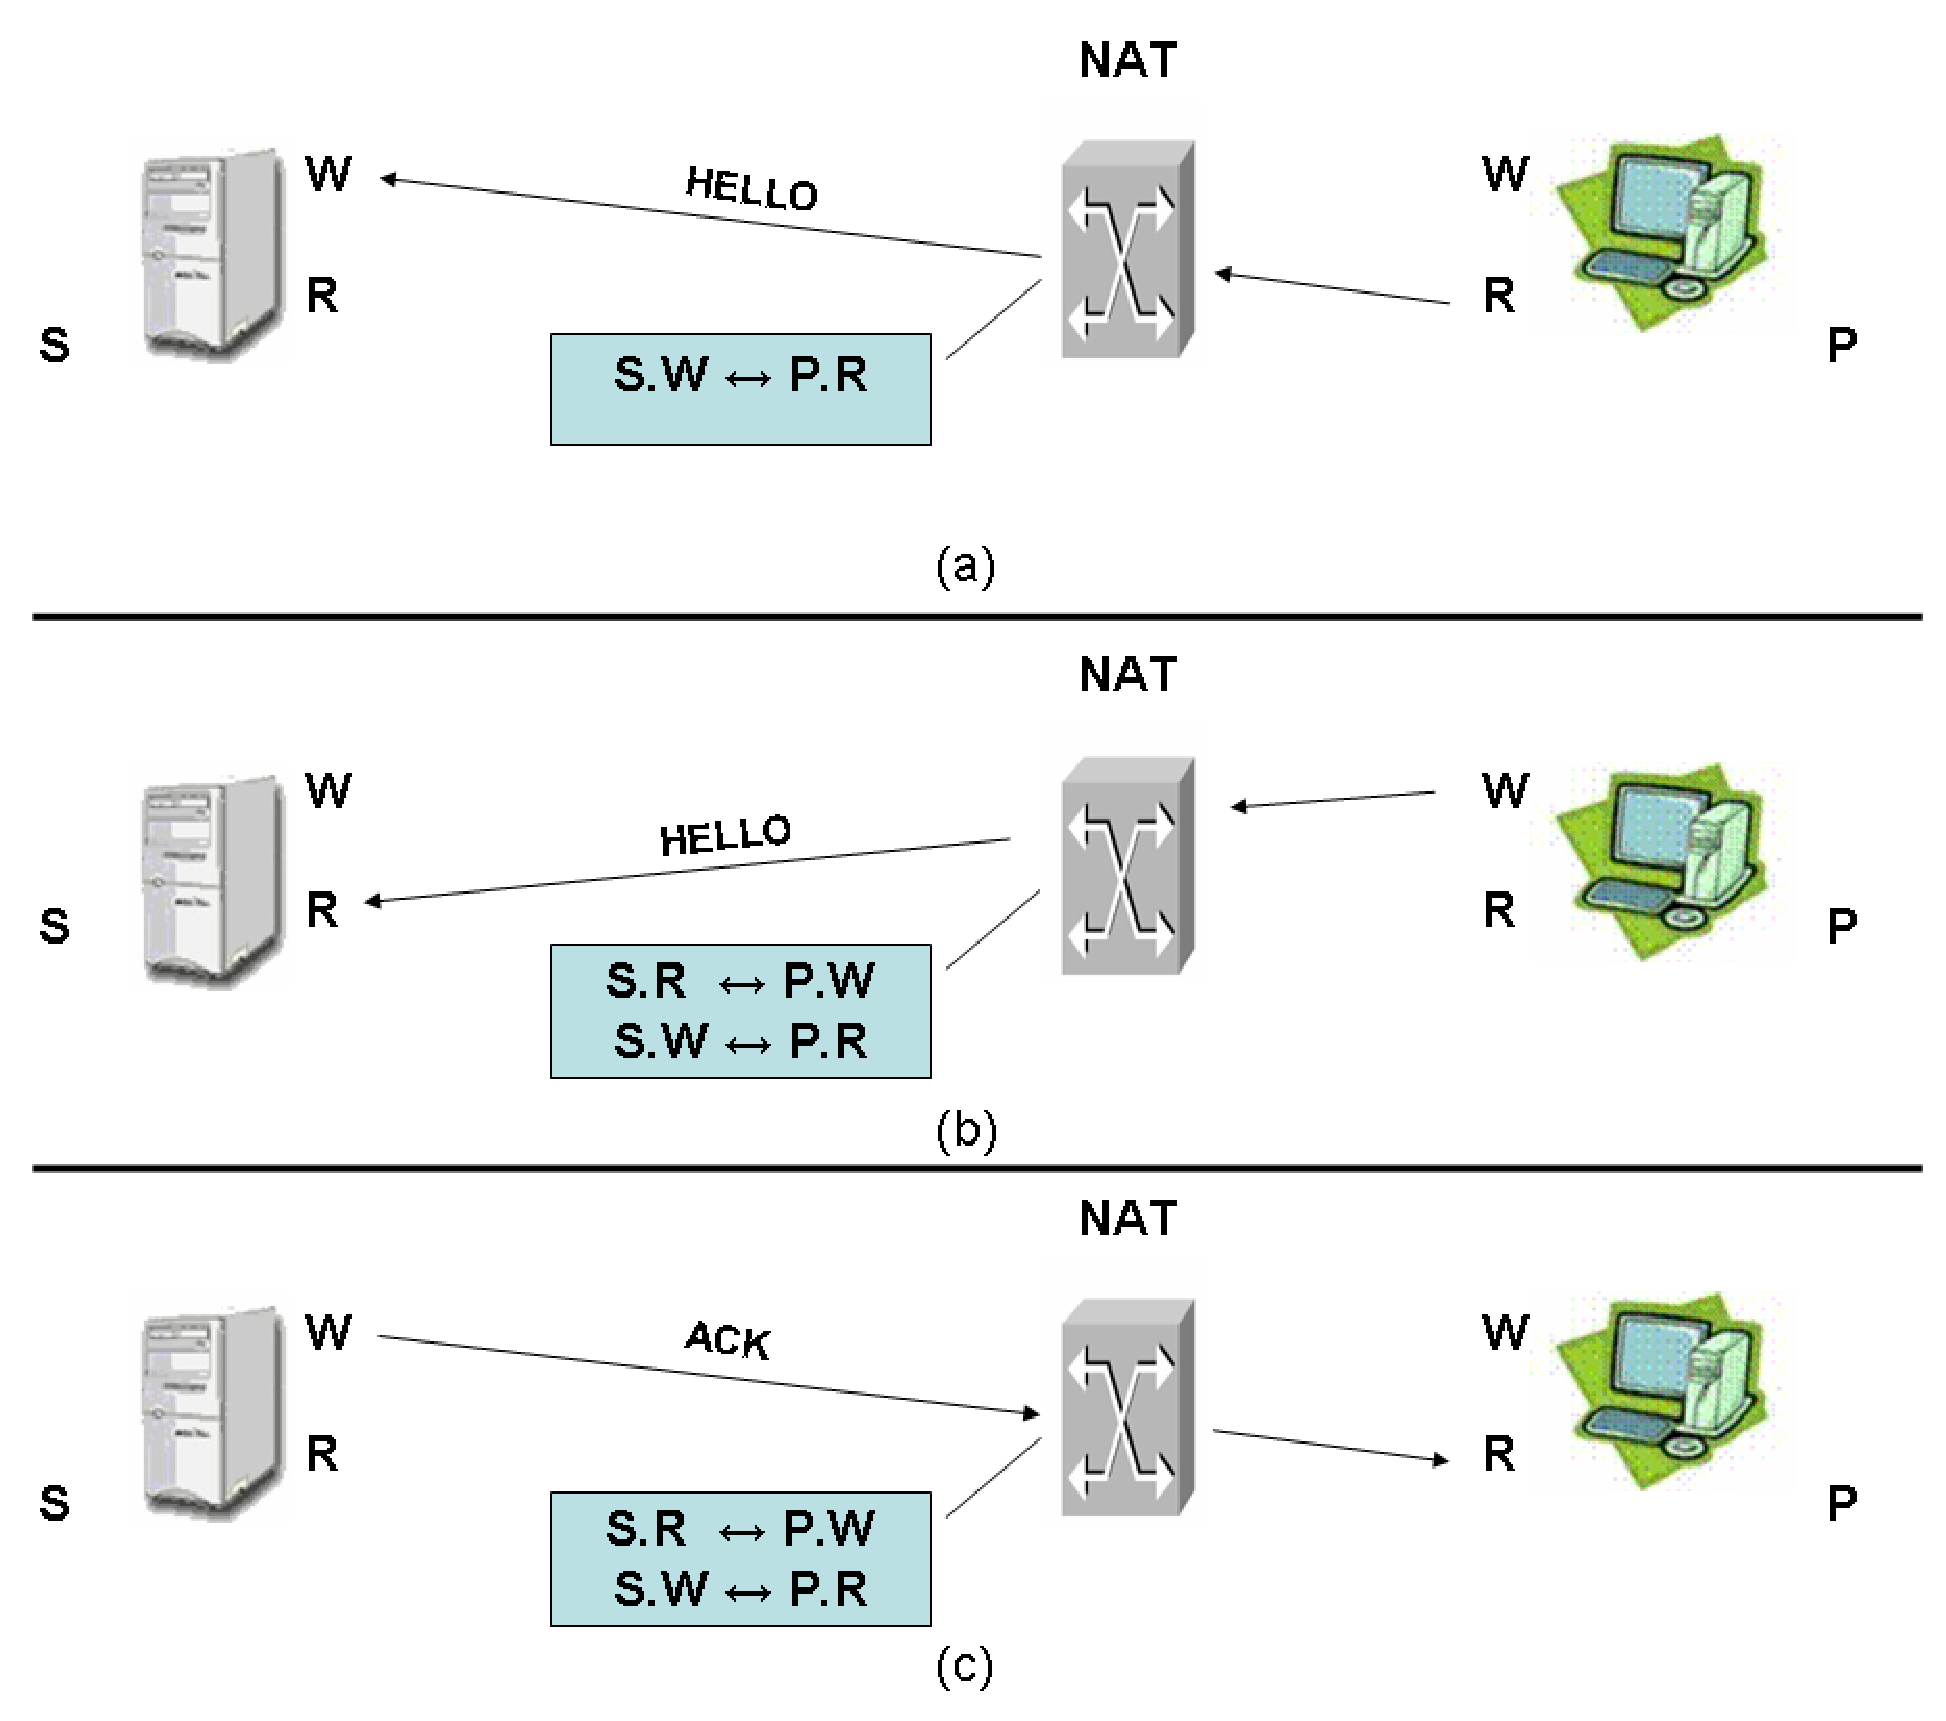
\includegraphics[scale=0.4]{first_phase.eps}
	\caption[Server-Peer NAT traversing]{Server-Peer NAT traversing}
	\label{fig:first_phase}
\end{figure}

Terminated this first phase, the new peer must permit others peers to communicate with it(??). If  the other peers are behind a NAT, they cannot be achievable from the new peer; is a server job to send a PPETP PUNCH command to those peers, while the new peer launch HELLO packet toward the other peer. When those peers receive the PUNCH command (with the address of the new peer), they starts the same procedure used in the first phase, but this time the send HELLO packets to the new peer address, but they cannot pass the NAT. To open a hole in the NAT the new peer send HELLO packets too; this permits the NAT be traversed.